\documentclass[tikz,border=2pt]{standalone}
\usepackage{times}
\usepackage[T1]{fontenc}
\usetikzlibrary{arrows.meta, positioning, fit, calc}

\begin{document}
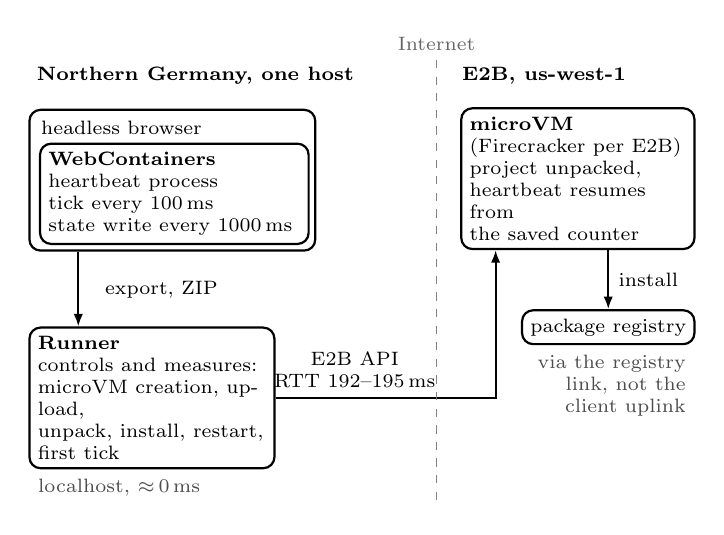
\begin{tikzpicture}[
  font=\scriptsize,
  box/.style={draw, thick, rounded corners, align=left, inner sep=3pt},
  zone/.style={font=\scriptsize\bfseries},
  note/.style={font=\scriptsize, align=left},
  flow/.style={-{Latex[length=1.6mm]}, thick}
]

\node[zone, anchor=west] at (0, 0) {Northern Germany, one host};
\node[zone, anchor=west] at (5.4, 0) {E2B, us-west-1};

\node[box, anchor=north west, text width=3.2cm] (wc) at (0.15, -0.85) {
  \textbf{WebContainers}\\
  heartbeat process\\
  tick every 100\,ms\\
  state write every 1000\,ms
};
\node[note, anchor=south west, inner sep=2pt] (chromiumtitle) at ($(wc.north west) + (-0.05, 0.02)$) {headless browser};
\node[draw, thick, rounded corners, fit=(chromiumtitle)(wc), inner sep=2pt] (chromium) {};

\node[note, anchor=north west] (export) at ($(chromium.south west) + (0.85, -0.25)$) {export, ZIP};

\node[box, anchor=north west, text width=2.9cm] (runner) at ($(chromium.south west) + (0, -0.95)$) {
  \textbf{Runner}\\
  controls and measures:\\ microVM creation, upload,\\ unpack, install, restart,\\ first tick
};

\draw[flow] (chromium.south -| 0.65, 0) -- (runner.north -| 0.65, 0);

\node[box, anchor=north west, text width=2.75cm] (vm) at (5.5, -0.4) {
  \textbf{microVM}\\
  (Firecracker per E2B)\\
  project unpacked,\\
  heartbeat resumes from\\
  the saved counter
};

\node[box, align=center, anchor=north east] (registry) at ($(vm.south east) + (0, -0.75)$) {package registry};
\node[note, anchor=north east, align=right, text=black!70] at (registry.south east) {via the registry\\ link, not the\\ client uplink};
\draw[flow] (registry.north |- vm.south) -- node[note, right] {install} (registry.north);

\coordinate (turn) at ($(vm.south west) + (0.45, 0)$);
\draw[flow] (runner.east) -- node[note, above, align=center, pos=0.36] {E2B API\\ RTT 192--195\,ms} (turn |- runner.east) -- (turn);

\node[note, anchor=north west, text=black!70] (localhost) at (runner.south west) {localhost, $\approx$\,0\,ms};

\draw[dashed, black!50] (5.2, 0.2) -- (5.2, 0 |- localhost.south);
\node[note, text=black!60, anchor=south, align=center] at (5.2, 0.2) {Internet};

\end{tikzpicture}
\end{document}
